% Название разделов -- все прописные
\section{ПОСТАНОВКА ЗАДАЧИ}

\subsection{Потребность в разработке электронных справочных материалов}

Врачи скорой помощи на каждый вызов вынуждены носить с собой много аппаратуры для обеспечения правильной диагностики и лечения пациентов. Это может быть как медицинское оборудование, так и различные инструменты, которые могут понадобиться в ходе работы. 


Несмотря на то, что в современном мире развитие технологий набирает оборот и медицинская аппаратура постоянно модернизируется, она все равно занимает много места и является достаточно тяжелой. Багаж работника скорой помощи весит около 6-7 кг. Там хранятся ампулы, таблетки, кровоостанавливающий жгут, зажим, пинцет и т.д.. Помимо этого врачи с собой носят карты вызовов скорой медицинской помощи. Они оформляются при каждом выезде бригады скорой помощи. Зачастую врачи работают в экстремальных ситуациях, где каждая секунда на счету. В таких условиях достаточно трудно и неудобно носить большое количество аппаратуры.


Также врачи с собой носят справочники. Они содержат информацию о диагнозах, протоколах оказания медицинской помощи и других медицинских стандартах. В этих справочниках указана информация о МКБ-кодировании, что позволяет врачам быстро и точно определить диагноз и выбрать наиболее подходящий протокол оказания медицинской помощи. Кроме того, справочные материалы содержат информацию о порядке оказания первой медицинской помощи в различных ситуациях, включая остановку сердца, инсульт, аллергические реакции и другие чрезвычайные ситуации. Поэтому врачам зачастую тяжело носить столько тяжелых вещей на каждый вызов.


Одним из возможных решений этой проблемы стали портативные планшеты. В настоящее время справочники для врачей скорой помощи часто представлены в электронном виде и могут быть доступны на планшетах и других мобильных устройствах. Это позволяет врачам быстро находить необходимую информацию и использовать ее для принятия решений на месте вызова, что повышает эффективность оказания помощи.
Вот еще несколько преимуществ портативных планшетов в сравнении с традиционными бумажными справочниками :
\begin{itemize}
    \item электронные справочники легко обновляются и актуализируются по мере появления новых медицинских стандартов и протоколов, поэтому врачи могут быть уверены в том, что они работают с актуальной на данный момент информацией;
    \item с электронными справочниками можно создавать резервные копии данных и сохранять их в защищенном хранилище. Это защищает информацию от потери или повреждения и обеспечивает возможность восстановления данных при необходимости.
\end{itemize}
	По итогу хочется заметить, что использование электронных справочников в предоставит врачам скорой помощи широкий спектр инструментов и функций для оптимизации процесса оказания помощи и улучшения качества медицинского обслуживания.

\subsection{Обзор существующих решений}

Существует достаточное количество как мобильных приложений, так и веб-приложений для врачей, которые могут помочь им в работе.

Проведем анализ и обзор некоторых из них, также выявим их недостатки:

\begin{enumerate}
    \item Мобильное приложение <<Справочник Врача: МКБ-10, РЛС>>
    Данное приложение является достаточно полезным и нужным инструментом для врачей, который помогает в работе. Приложение включает в себя данных о лекарственных средствах, включая информацию о препаратах, их дозировках, побочных эффектах, взаимодействиях и противопоказаниях. Врачи могут использовать эту информацию для подбора правильного лекарственного средства для пациента, оценки безопасности и эффективности лекарств и предотвращения нежелательных реакций. Также там присутсвуют разделы об анализах, справочнике МКБ.Врачи могут использовать это для поиска и проверки правильности диагнозов, а также для стандартизации и согласования кодов диагнозов для медицинской документации и статистики.

    На рисунке~\ref{fig:fig03} приведен главный экран мобильного приложения <<Справочник Врача: МКБ-10, РЛС>>.
    
    \begin{figure}
        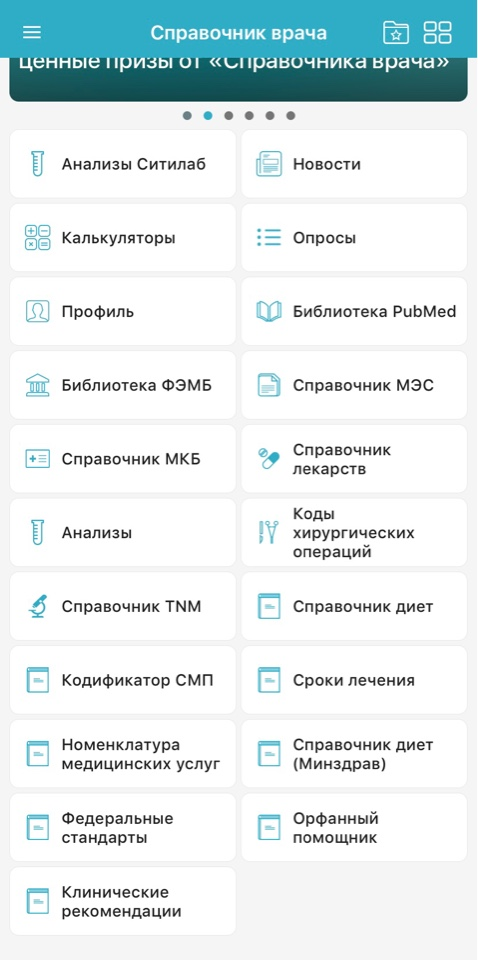
\includegraphics[scale=0.6]{styles/diploma/inc/prog1.jpeg}
        \caption{Главная страница приложения <<Справочник Врача: МКБ-10, РЛС>>}
        \label{fig:fig03}
    \end{figure}

    На рисунке~\ref{fig:fig04} приведено боковое меню мобильного приложения <<Справочник Врача: МКБ-10, РЛС>>.
     \begin{figure}
        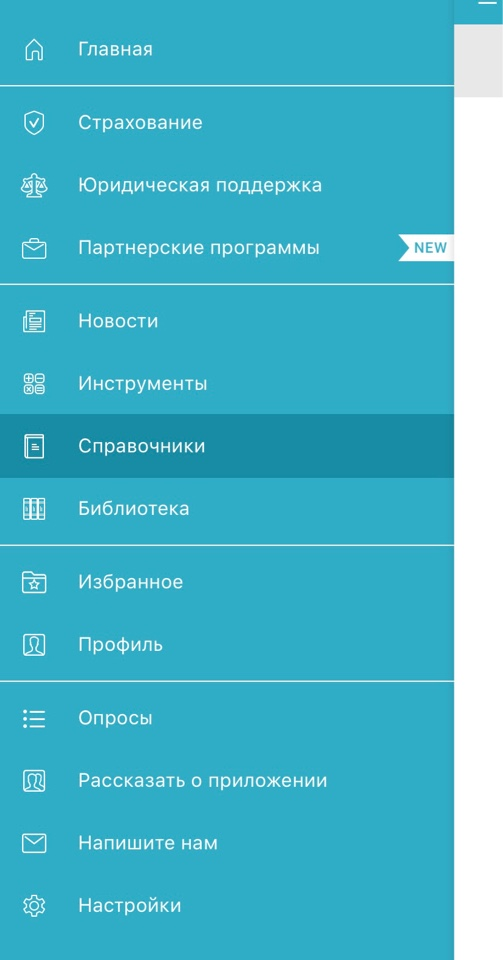
\includegraphics[scale=0.6]{styles/diploma/inc/prog2.jpeg}
        \caption{Боковое приложения <<Справочник Врача: МКБ-10, РЛС>>}
        \label{fig:fig04}
    \end{figure}
    
    Недостатки данного приложения:
    \begin{itemize}
        \item врач скорой помощи не сможет заполнять и хранить в нем карты пациентов. Т.е. это приложение предоставляет только справочную информацию;
        \item неудобный и избыточный интерфейс. Интерфейс перегружен: запутанное меню, сложная структура приложения, то есть для поиска нужной информации нужно затрачивать больше времени. Излишняя информация: (новости, опросы) на главной странице приложения.

        Плохая организация данных: если ты зашел в раздел МКБ, то для того, чтобы попасть в другой раздел, сначала необходимо перейти в боковое меню (рисунок~\ref{fig:fig04}  ), затем перейти на главную страницу, после чего выбрать нужный раздел (т.е. нет удобной навигации по разделам);
        
        \item в приложении не предусмотрена какая-либо информация об алгоритмах оказания медицинской помощи.
    \end{itemize}
    \item Бот в Telegram Paramedic
    Предоставляет довольно ограниченный функционал. Там можно получить информацию только по алгоритмам оказания скорой помощи, кодам МКБ и порядку заполнения карты вызова.
    
    На рисунке~\ref{fig:fig05} приведены справочные материалы, которые может предосталвять Telegram bot <<Paramedic>> в Москве.
    \begin{figure}
        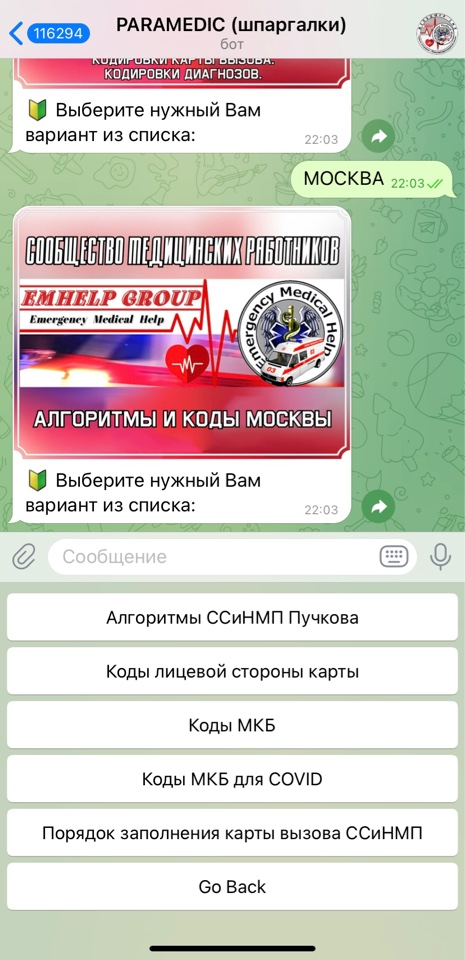
\includegraphics[scale=0.6]{styles/diploma/inc/prog2_1.jpeg}
        \caption{Telegram bot <<Paramedic>>}
        \label{fig:fig05}
    \end{figure}

    На рисунке~\ref{fig:fig06} приведены разделы медицины, которые содержит бот.Также показано, в каком виде он предоставляет информацию по алгоритмам.

     \begin{figure}
        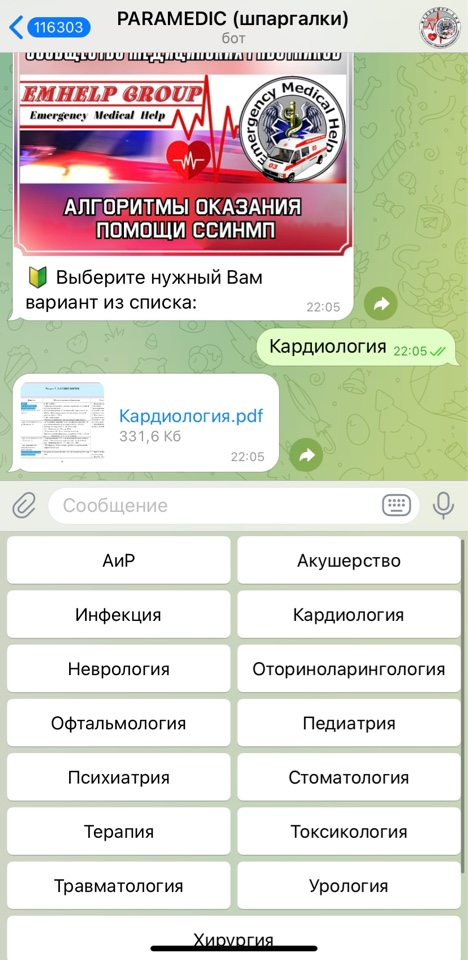
\includegraphics[scale=0.6]{styles/diploma/inc/prog2_2.jpeg}
        \caption{В каком виде представлена информация по алгоритмам в Telegram bot <<Paramedic>>}
        \label{fig:fig06}
    \end{figure}

    Недостатки данного решения:
    \begin{itemize}
        \item как и в преложении, описанном выше, врач скорой помощи не сможет заполнять и хранить в нем карты пациентов, т.е. этот бот предоставляет только справочную информацию;
        
        \item в приложении есть информация по алгоритмам, которые можно найти по разделу. После чего появляется PDF - документ, в котором содержатся коды МКБ и необходимые действия для оказания помощи.

        Это не очень удобно по нескольким причинам:
         \begin{itemize}
            \item PDF-документы могут быть неудобными для чтения на мобильных устройствах или экранах с небольшим размером. Они могут требовать масштабирования или скроллинга, чтобы прочитать весь контент, что может затруднить навигацию и восприятие информации;
            \item PDF-документы обычно являются статичными и не предоставляют интерактивные возможности, такие как поиск или динамическое обновление информации. Это может затруднять быстрый доступ к нужным данным или усложнять поиск конкретных кодов МКБ или действий;
            \item так как информация предоставляется в виде отдельного PDF-документа, пользователю может потребоваться переключаться между приложением и приложением для чтения PDF-файлов, что может быть неудобным и требовать дополнительных действий.
         \end{itemize}
    \end{itemize}
    \item Веб-приложение <<Рубрикатор клинических рекомендаций>>
    Это довольно ценный ценный инструмент для врачей и медицинского персонала, предоставляющий информацию о клинических рекомендациях, алгоритмах действия врача, справочниках, также в нем можно найти данные о разработке клинических рекомендаций. Этот инструмент содержит в себе только информацию справочного характера. Таким образом, он не предоставялет возможность заполнения карты пациента для работников скорой помощи. 

    На рисунке~\ref{fig:fig07} приведен главный экран веб-приложения <<Рубрикатор клинических рекомендаций>>.
        \begin{figure}
        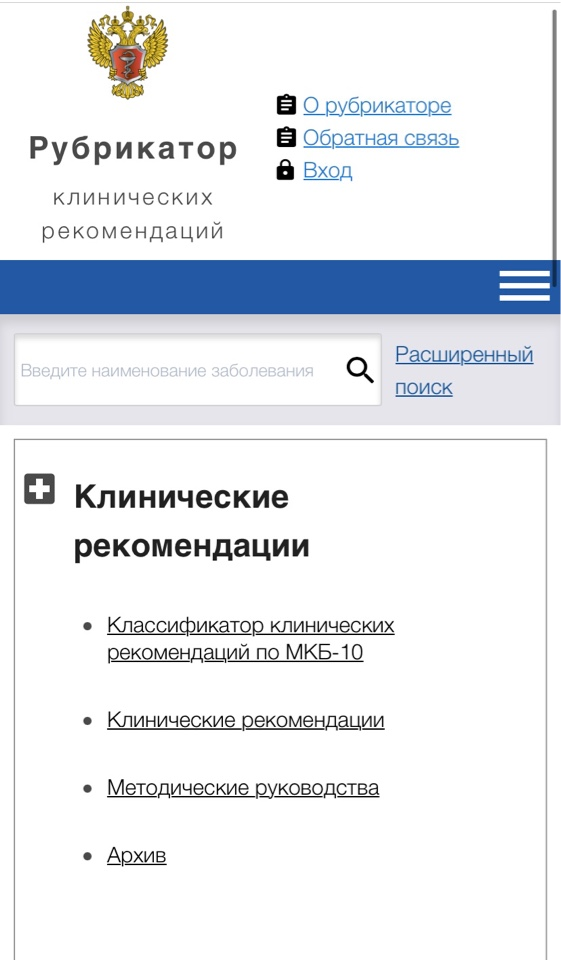
\includegraphics[scale=0.6]{styles/diploma/inc/prog3_1.jpeg}
        \caption{Главная страница веб-приложения <<Рубрикатор клинических рекомендаций>}
        \label{fig:fig07}
    \end{figure}
    
    На рисунке~\ref{fig:fig08} приведен пример алгоритма действий врача из <<Рубрикатора клинических рекомендаций>>.

     \begin{figure}
        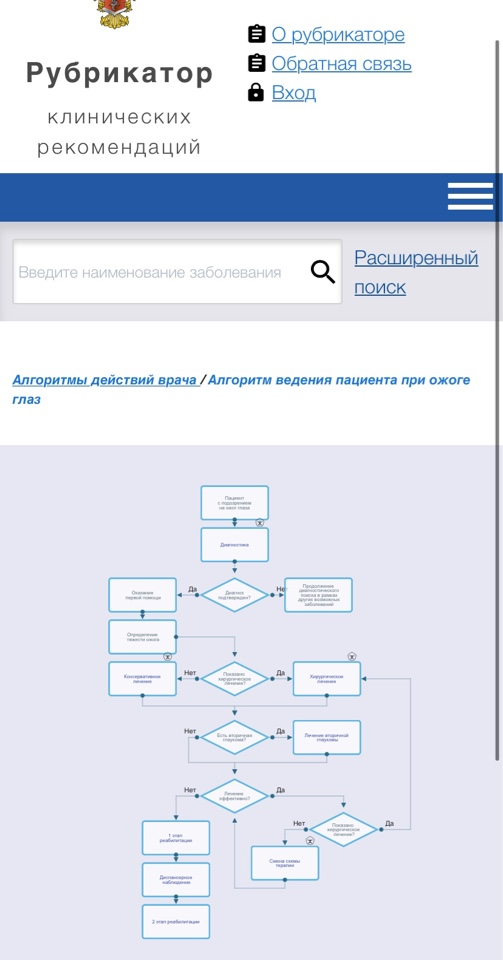
\includegraphics[scale=0.6]{styles/diploma/inc/prog3_2.jpeg}
        \caption{Алгоритм действий врача из <<Рубрикатора клинических рекомендаций>>}
        \label{fig:fig08}
    \end{figure}
    Недостатки данного решения:
    
    \begin{itemize}
        
        \item в приложении есть информация по алгоритмам, которые можно найти по разделу. Алгоритмы представлены в виде блок-схем.

        Это не очень удобно по нескольким причинам:
         \begin{itemize}
            \item блок-схемы могут быть слишком упрощенными, особенно в сложных алгоритмах. Иногда сложные шаги или логические условия могут быть трудно представить в виде простых блоков, что может привести к потере деталей или понимания алгоритма;
            \item в больших и сложных алгоритмах блок-схемы могут занимать много места и становиться запутанными. Это может затруднить чтение и понимание всего алгоритма на одном экране, особенно если алгоритм состоит из большого числа шагов;
            \item блок-схемы могут иметь ограниченные возможности в описании сложных условий, итераций и других аспектов алгоритма. Они могут не быть подходящим инструментом для полного описания всех деталей и особенностей сложных алгоритмов.
         \end{itemize}
    \end{itemize}
\end{enumerate}

\subsection{Техническое задание на разработку}

Таким образом, в результате данной работы должен быть реализован функционал, который содержит информацию, предоставляющую алгоритмы оказания медицинской помощи. 

Алгоритмы представляют собой кодировку МКБ и определнный диагноз, который содержит информацию о различных аспектах этого диагноза.
Одним из ключевых элементов алгоритма является название диагноза, которое явно указывает на медицинское состояние или проблему со здоровьем, которую алгоритм описывает. Название диагноза обычно основывается на систематической классификации и является основным способом идентификации конкретного алгоритма.
Кроме того, алгоритмы содержат информацию о случаях, связанных с данным диагнозом. В каждом случае описываются особенности и характеристики заболевания или состояния, включая симптомы.

Одной из важных составляющих алгоритмов является объем помощи и рекомендации. Здесь описываются конкретные процедуры, методы и рекомендации для оказания медицинской помощи пациенту с данным диагнозом. Это может включать назначение лекарств, физиотерапию и другие медицинские мероприятия.

Наконец, в алгоритмах также присутствует информация о тактике, которая определяет стратегию и последовательность действий после оказания медицинской помощи. Тактика может варьироваться в зависимости от сложности и характера диагноза, а также от общего состояния пациента.

На рисунке~\ref{fig:fig13} приведен пример алгоритма  оказания неотложной медицинской помощи.

     \begin{figure}
        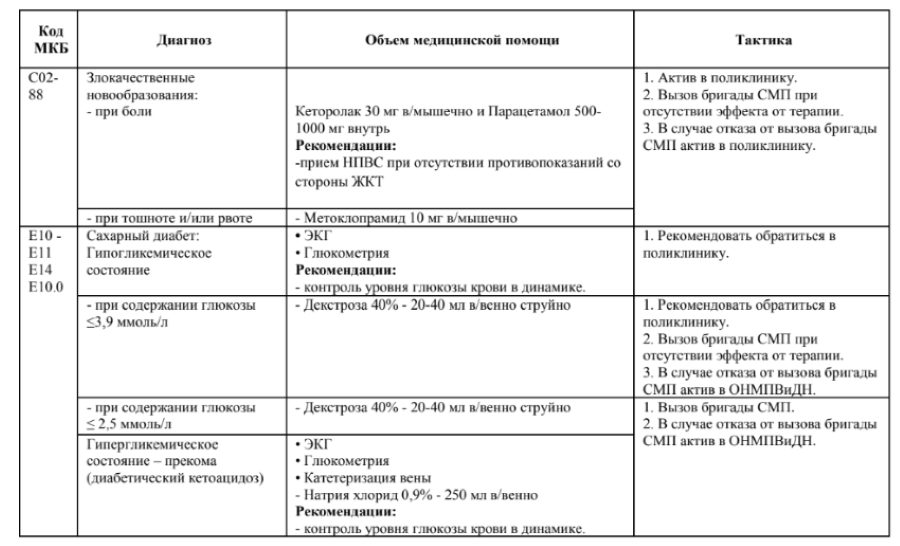
\includegraphics[scale=0.6]{styles/diploma/inc/algo1.png}
        \caption{Пример структуры алгоритма}
        \label{fig:fig13}
    \end{figure}

Требования к функционалу:

\begin{itemize}
    \item понятный пользовательский интерфейс. Разработать пользовательский интерфейс веб-приложения, включающий поисковую строку для ввода кода МКБ и отображение результата поиска в виде названия диагноза, тактики, рекомендаций и медицинской помощи;
    \item поиск по коду МКБ. Реализовать механизм поиска, который позволяет вводить код МКБ и получать соответствующую информацию о диагнозе и связанной помощи;
    \item отображение информации. Предоставить четкое и понятное отображение названия диагноза, тактики, рекомендаций и медицинской помощи для каждого найденного диагноза;
    \item контроль. Реализовать проверку всех оказанных врачом действий, связанных с оказанием медицинской помощи, с помощью checkboxов. Если выбраны не все действия по оказанию медецинской помощи и врач пытается перейти в другой раздел заполнения медицинской карты, то вылезает сообщение о том, что медицинскому работнику стоит убедиться, что все действия выполнены и он уверен в том, что хочет покинуть данную страницу.
\end{itemize}
